\documentclass{beamer}


% Load essential packages
\usepackage{hyperref} % Only load once to avoid conflicts
\usepackage{stile}
\usepackage{subcaption}
\usepackage{tcolorbox}
\usepackage[font=scriptsize,skip=1pt]{caption}
\usepackage[T1]{fontenc}
\usepackage{csquotes}
\usepackage[backend=biber, style=authoryear, maxnames=3, minnames=1, abbreviate=false, date=long, url=false, isbn=false, doi=false]{biblatex}
\addbibresource{lecture6/bib.bib} % Ensure this matches your bibliography file name

\interfootnotelinepenalty=10000

\usepackage{latexsym, amsmath, xcolor, multicol, booktabs, calligra}
\usepackage{graphicx, pstricks, listings, stackengine}

% Hyperref setup
\hypersetup{
    hidelinks,
    colorlinks=true,
    linkcolor=black,
    citecolor=blue,
    urlcolor=black
}

% Font theme for Beamer
\usefonttheme[onlymath]{serif}

% Custom definitions
\def\cmd#1{\texttt{\color{red}\footnotesize $\backslash$#1}}
\def\env#1{\texttt{\color{blue}\footnotesize #1}}
\definecolor{deepblue}{rgb}{0,0,0.5}
\definecolor{deepred}{rgb}{0.6,0,0}
\definecolor{deepgreen}{rgb}{0,0.5,0}
\definecolor{halfgray}{gray}{0.55}

% Beamer color settings
\setbeamercolor{block title}{bg=blue!70!white, fg=white}
\setbeamercolor{block body}{bg=blue!10!halfgray, fg=white}
\setbeamercolor{section in head/foot}{fg=white}
\setbeamercolor{subsection in head/foot}{fg=white}
\setbeamercolor{title in head/foot}{fg=white}


% Listings settings for code highlighting
\lstset{
    basicstyle=\ttfamily\small,
    keywordstyle=\bfseries\color{deepblue},
    emphstyle=\ttfamily\color{deepred},
    stringstyle=\color{deepgreen},
    numbers=left,
    numberstyle=\small\color{halfgray},
    rulesepcolor=\color{red!20!green!20!blue!20},
    frame=shadowbox,
}

% Title page info
\author{Freya Rubel}
\title{Trade, Migration and Global Challenges}
\subtitle{Protectionism and Trade Wars}
\institute{}
\date{27.11.2025}

\graphicspath{{lecture6/}}

\begin{document}

\begin{frame}
    \titlepage
\end{frame}

\begin{frame}
    \tableofcontents[sectionstyle=show, subsectionstyle=show/shaded/hide, subsubsectionstyle=show/shaded/hide]
\end{frame}

\section{Barriers to Trade (Protectionism)}
\begin{frame}{Introduction}
    Goods (and services) do not circulate freely around the world.
    \begin{itemize} \small
        \item Protectionism is understood as trade-reducing policies that impose barriers to trade.
        \item Subsidies, too, can be considered protectionist measures when they aim at decreasing imports. % can you explain why subsidizing the own economy is considered protectionist? answer: you are creating an unfair/artificial advantage of your own industry over the foreign industry, thereby hurting imports from foreign industries into your country
    \end{itemize}
    Trade restrictions
    \begin{itemize} \small
        \item Taxes on trade flows e.g, \textbf{tariffs}
        \item Non-tariff barriers to trade (NTBs)
    \end{itemize}
\end{frame}

\begin{frame}{Tariff Formation}
    What determines the formation and level of a tariff?
    \begin{itemize}
        \item Standard motivation: Trade liberalization can hurt certain domestic markets. 
        \item The state can have an incentive to impose a tariff since it generates revenue for the government.
        \item Tariffs can also address market distortions and thereby increase efficiency (second-best solution).
    \end{itemize}
\end{frame}

\begin{frame}[t]{Graphical Example - Import Tariff}
\small
    Assumption: The home country is a small country in which supply and demand conditions do not affect international prices.
   
\end{frame}

\begin{frame}{Import Tariff - Takeaways}
\small
    \begin{itemize}
    \item In autarky, domestic price and quantity is determined by domestic supply and demand
    \item Under free trade, domestic consumers are winning if the world market price is below the domestic equilibrium price, and domestic producers are losing. The overall welfare is increasing.
    \item When imposing a tariff, overall welfare is shrinking compared to the free trade scenario because domestic consumers are losing. Domestic producers are gaining, and the government is gaining as well. 
    \item Imposing a tariff is reducing the quantity of foreign products imported because their price to the domestic consumers is increasing.
    \end{itemize}
\end{frame}

\begin{frame}{Non-Tariff Barriers to Trade}
Types:
     \begin{itemize} \small
        \item \textbf{Quotas:} Limits on the quantity of goods that can be imported.
        \item \textbf{Standards and Regulations:}
        \begin{itemize} \footnotesize
            \item Sanitary and Phytosanitary (SPS) Measures. \textcolor{gray}{Examples: Ban on the import of hormone-treated beef, limit on the residue of pesticides detectable in food products, quality standards.}
            % world trade organisation allows member states to impose their own rules on the food safety as well as animal and plant safety regulation and standards. There are international guidelines that countries are supposed to follow but they can also impose their own standards if they see a scientific basis or it (can't be arbitrary and 
            \item Technical Barriers to Trade (TBT).  \textcolor{gray}{Examples: Requirement to print nutritional values on food items, the language of labelling, energy efficiency standards.} % exporters must redesign their packaging, which is not only a pain but costs real money, so it's increasing the costs of the goods that are exported
        \end{itemize}
        \item \textbf{Subsidies:} Governments' financial support to domestic industries.
        \item \textbf{Customs Delays and Bureaucracy:} Lengthy procedures at borders. % imposes a cost, even though it is not a monetary cost
    \end{itemize}
\end{frame}

\begin{frame}[t]{Graphical Example - Import Quota}
\small
    Assumption: The home country is a small country in which supply and demand conditions do not affect international prices.
  
\end{frame}

\begin{frame}[t]{Import Quota - Takeaways}
\small
    \begin{itemize}
    \item In autarky, domestic price and quantity are determined by domestic supply and demand
    \item Under free trade, domestic consumers are winning if the world market price is below the domestic equilibrium price, and domestic producers are losing. The overall welfare is increasing.
    \item When governments impose a quota (free of charge), overall welfare is shrinking compared to the free trade scenario because domestic consumers are losing. Domestic producers are gaining. Whether foreign producers are gaining or loosing, depends on the size of the quota. 
    \item Imposing a quota is reducing the quantity of foreign products imported only if the quota is binding, meaning the quota is smaller than the number of units imported in a free trade scenario without a quota.
    \end{itemize}
\end{frame}


\begin{frame}{Which Industries Need Protection? (5 min)}
    \begin{Large}
        Discuss with a partner: \vspace{0.2cm}\\
        If you were in charge of an economy, which of your industries (product group) would you protect the most (impose trade barriers on imports of competing foreign products) and why? Which conditions/factors does your answer depend on?
    \end{Large} \vspace{0.2cm}\\
    \textcolor{gray}{Examples: Wood, Fuels, Minerals, Vegetables, Food Products, Chemicals, Plastics, Metals, ...}
\end{frame}

\begin{frame}{Tariffs across Industries}
    \begin{figure}
        \centering
        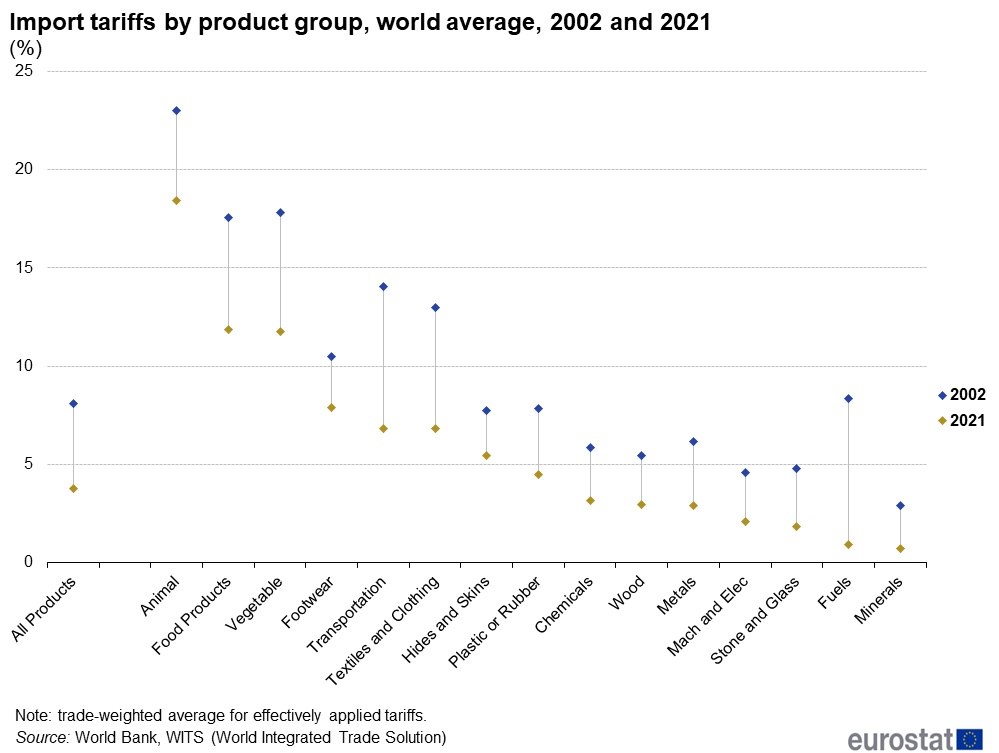
\includegraphics[width=0.9\linewidth]{Import_tariffs_by_product_group,_world_average,_2002_and_2021.png}
        \label{fig:enter-label}
    \end{figure}
\end{frame}

\begin{frame}{When is it Rational/Efficient to use Tariffs?}
    \textbf{Key Arguments}
\begin{itemize} \small
    \item \textbf{Protectionist Interests:}
    \begin{itemize} \footnotesize
        \item Protect an emerging industry from the competition of more advanced foreign market participants.
        \item Protecting inefficient but critical industries (pharmaceuticals, food security)
    \end{itemize}
    \item \textbf{Distributive Justice:}
    \begin{itemize} \footnotesize
        \item Even if overall welfare increases, it's hard to put a price on an equal society. 
    \end{itemize}
\end{itemize}
\textbf{Modern Perspective}
\begin{itemize} \small
    \item \textbf{Coordinated Tariffs:}
    \begin{itemize} \footnotesize
        \item Tariffs on high-emission goods can significantly curb carbon emissions.
        \item Example: EU Carbon Border Adjustment Mechanism (CBAM) 
    \end{itemize}
\end{itemize}
\end{frame}


\begin{frame}{Key Takeaway}
    \begin{tcolorbox}
        \begin{itemize}
            \item Tariffs are a type of protectionist trade barrier.
                \item Other non-tariff trade barriers include quotas, licenses, and standardization, all seeking to make foreign goods more expensive or available in a limited supply. 
    \item While protectionism benefits certain domestic sectors, economists generally agree that free trade policies in a global market are ideal for the overall economy.
    \item Tariffs are paid by importers and domestic consumers and not the exporting country, but they have the effect of raising the relative prices of imported products, which reduces demand for foreign products and thereby hurts the foreign economy.
        \end{itemize}
    \end{tcolorbox}
\end{frame}

\begin{comment}
\section{Tariffs as Second-Best Instruments}
\begin{frame}{The Concept of the "Second-Best"}
    \textbf{Definition:} \\
    The \textit{Theory of the Second-Best} (\cite{lipsey_general_1956}) states that if one optimal condition for economic efficiency cannot be satisfied, attempting to satisfy other optimal conditions does not necessarily lead to the second-best outcome. \vspace{0.15cm}\\
    \textcolor{deepblue}{Key Insight:} Removing one distortion in the presence of other distortions might reduce, not improve, overall efficiency. \vspace{0.15cm}\\
    \textbf{Perfect competitive market}
    \begin{itemize} \footnotesize
        \item Large (infinite) number of buyers and sellers
     \item Homogenous/identical goods 
        \item No barriers to entry or exit for producers
        \item Complete information
        \item No externalities
        \item Well-defined property rights
        \item No returns to scale 
        \item No state intervention
    \end{itemize}
\end{frame}

\begin{frame}{Market Failures and Government Intervention - Negative Externality}
Example: The production of each unit of a good imposes a cost (pollution) on the consumers that is not incorporated in the private cost function of the suppliers.
    \begin{figure}
        \centering
        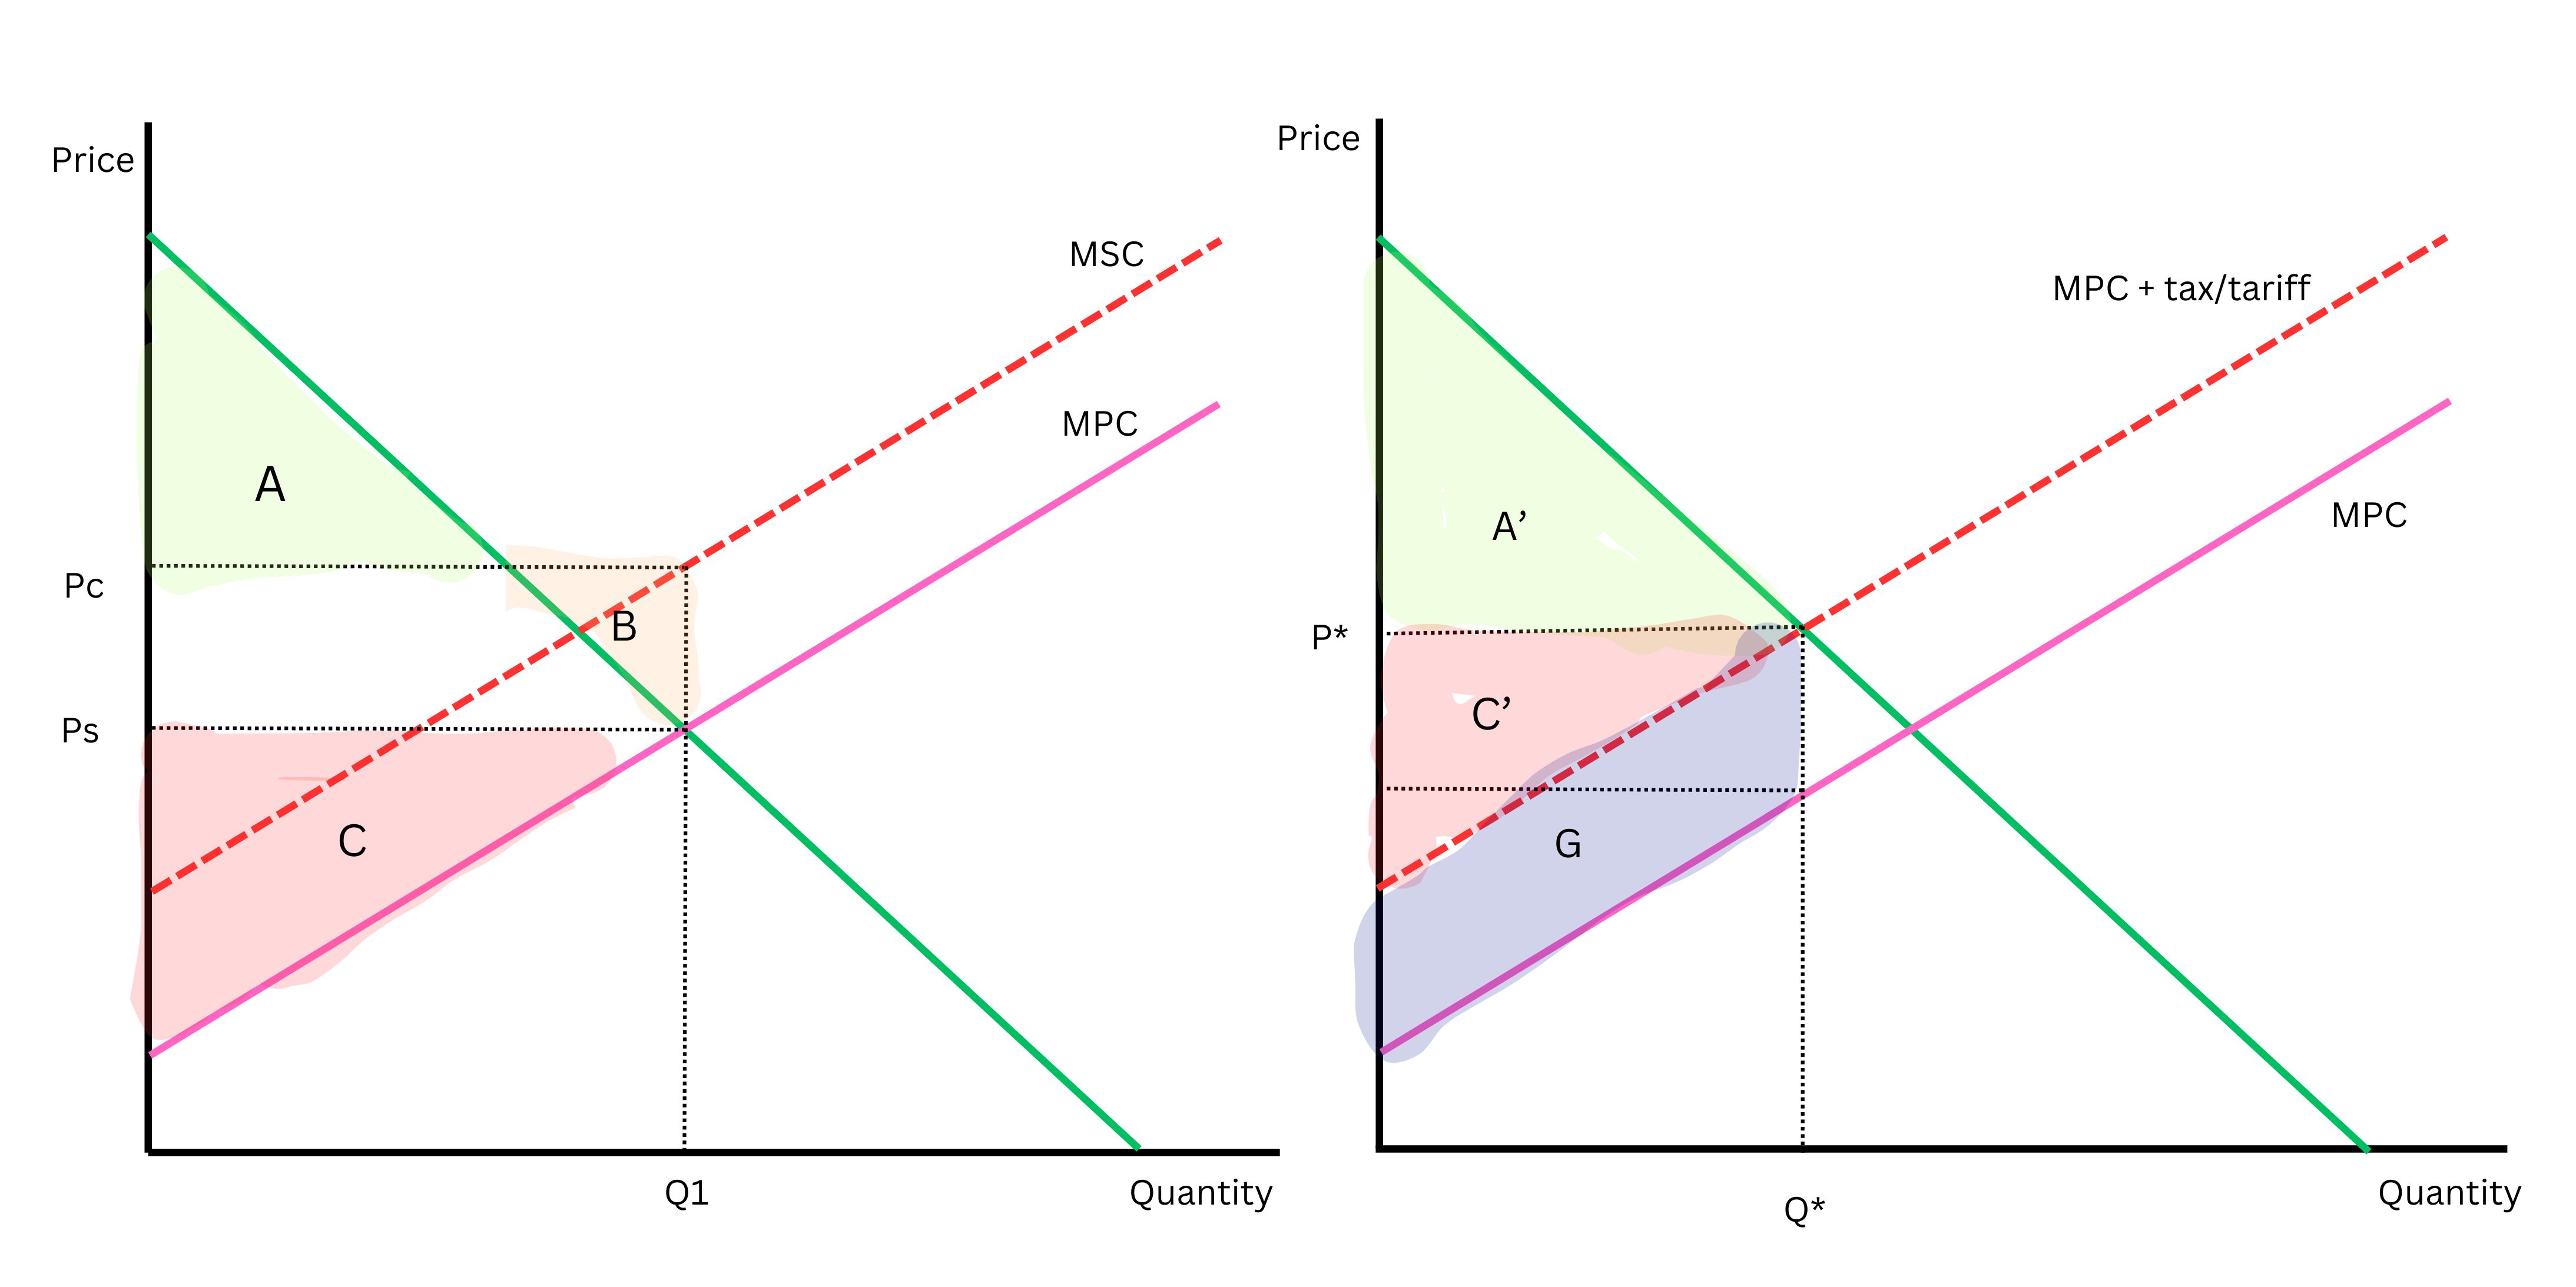
\includegraphics[width=\linewidth]{Pigouvian tax.png}
        \label{fig:enter-label}
    \end{figure}
\end{frame}

\begin{frame}{When is it Rational/Efficient to use Tariffs?}
    \begin{itemize}
        \item When we live in a world with imperfect competition and monopolies can take advantage of economies of scale.
        \begin{itemize}
            \item Global perspective: subsidies can be welfare improving, and we should encourage subsidies that foster competition between large multinational corporations.  
        \end{itemize}
        \item When we live in a world with externalities. 
        \begin{itemize}
            \item It makes sense to use tariffs if...
            \begin{itemize}
                \item pollution is elastic to output
                \item output is elastic to exports
                \item exports are elastic to tariffs
            \end{itemize}
            \item Example: EU Carbon Border Adjustment Mechanism (CBAM) as a carbon-tariff % I have presented the concept already in the class on Trade and Migration. Who remembers what the CBAM is?
        \end{itemize}
    \end{itemize}
\end{frame}
\end{comment}



\section{Trade Wars}

\begin{frame}{Introduction}
        A trade war occurs when countries impose tariffs or other trade barriers on each other in retaliation because one perceives unfair trade practices.
\begin{figure}
    \centering
    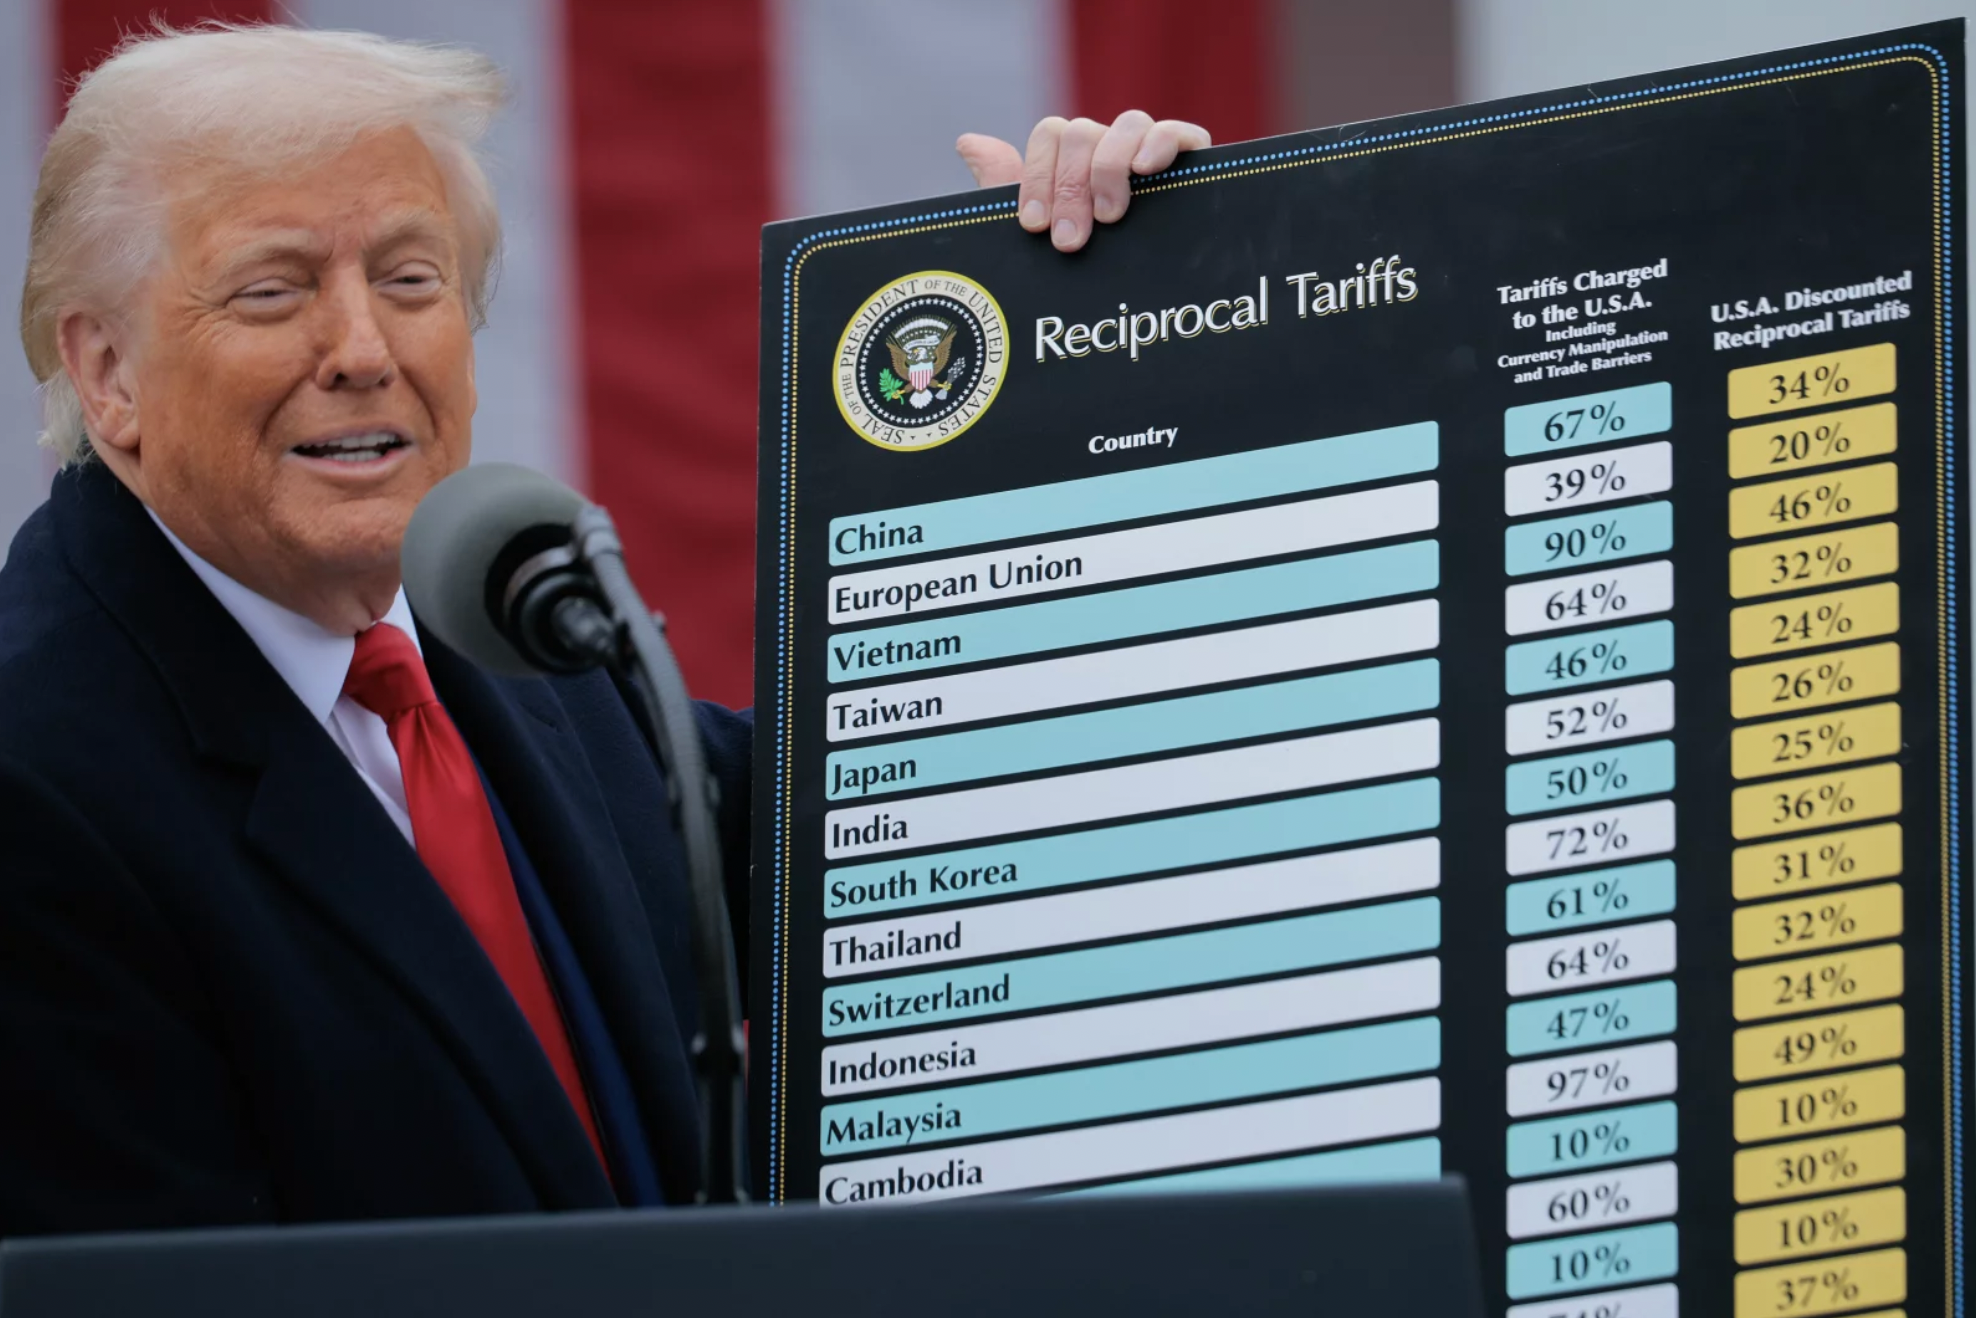
\includegraphics[width=0.6\linewidth]{trump with tariffs .png}
    %\caption{Pop culture moment of 2025}
    \label{fig:placeholder}
\end{figure}
\end{frame}

\begin{frame}{Tit-for-tat}
            \begin{itemize} \small
                \item Retaliation: a country imposes trade measures of similar magnitude in response to actions taken by another country.
                \item Can escalate tensions (spiral) and harm both economies if prolonged.
            \end{itemize}
        Common tools of a trade war include:
        \begin{itemize} \small
            \item \textbf{Tariffs:} Taxes on imported goods.
            \item \textbf{Quotas:} Limits on the quantity of imports.
            \item \textbf{Subsidies:} Financial support for domestic industries.
            \item \textbf{NTBs:} Non-Tariff Barriers, such as regulations or licensing requirements.
        \end{itemize}
\end{frame}

\begin{frame}{US Trade Deficit 1997-2021}
$$GDP=C+I+G+(X-M)$$ \pause
\begin{figure}
    \centering
    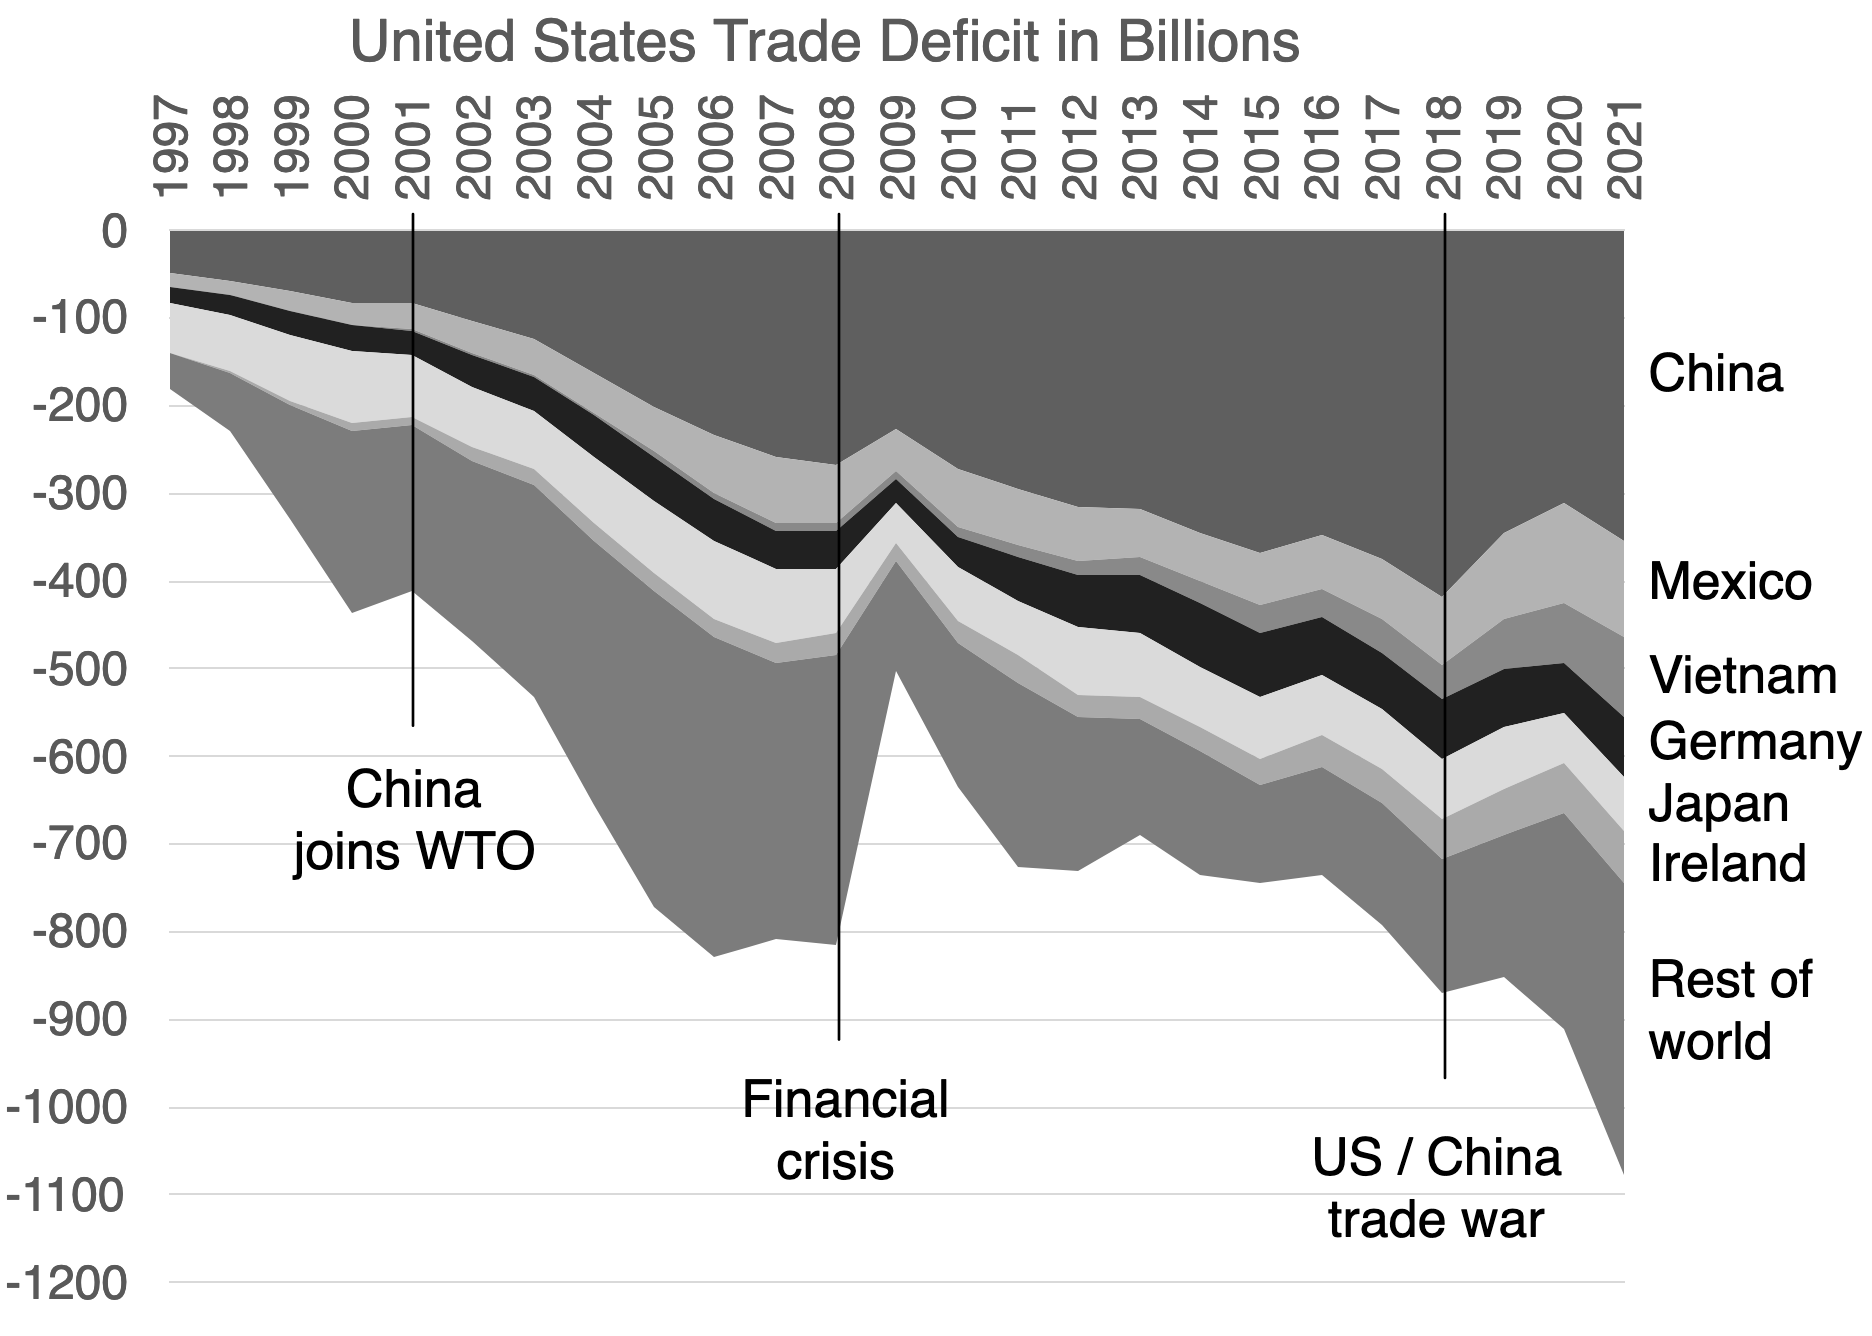
\includegraphics[width=0.8\linewidth]{US Trade Deficit.png}
    \caption{Source: US Census Bureau}
    \label{fig:enter-label}
\end{figure}
\end{frame}

\begin{frame}{Trump Tariffs - Explained}
\small
\textbf{Calculation of ''Tariffs Charged to the USA''}
    $$\Delta \tau_i=\frac{x_i-m_i}{\epsilon \times \varphi \times  m_i} = \frac{x_i - m_i}{m_i}$$
    \begin{itemize} \scriptsize
        \item [$\epsilon$] Elasticity of import demand (set at 4)
        \item [$\varphi$] Price passthrough (set at 0.25)
    \end{itemize} \pause
    ''Tariffs Charged to the USA'' = trade deficit as a percentage of imports
    \begin{quote}
    \textit{
        ''[...] The model they use is based on the concept that the trade deficit that we have with any given country is the sum of all the unfair trade practices, the sum of all cheating.''} \begin{footnotesize}
            (White House Official on April 2, 2025)
        \end{footnotesize}
    \end{quote}
    
\end{frame}

\begin{frame}{Example: US-China Trade War 2018 Background}
    \textbf{Background:}
\begin{itemize} \small
    \item Began in 2018 under the Trump administration.
    \item U.S. accused China of unfair trade practices, including:
    \begin{itemize} \footnotesize
        \item Intellectual property theft and forced technology transfers.
        \item Massive trade imbalance. 
        \item State subsidies to Chinese industries.
    \end{itemize}
    \item U.S. imposed tariffs on Chinese goods; China retaliated with similar measures.
\end{itemize}
\textbf{Key Measures:}
\begin{itemize} \small
    \item U.S. tariffs on steel, electronics, machinery, later also consumer goods and furniture.
    \item Chinese retaliated with tariffs on U.S. agricultural products (soybeans, pork, etc.), thereby targeting particular constituencies $\implies$ regional inequalities.
\end{itemize}
\end{frame}

\begin{frame}{Phases of the Trade War}
    \textbf{\small U.S. Provocation:}
    \begin{itemize} \footnotesize
        \item 07.02.2018: 30\% tariff on solar panel imports
        \item 23.03.2018: 25\% tariff on steel imports and 10\% tariff on aluminium imports
    \end{itemize}
    \textbf{\small Retaliation from China:}
    \begin{itemize} \footnotesize
        \item 02.04.2018: 15-25\% retaliatory tariffs on US products (incl. fruit, pork, recycled aluminium, steel tubing)
    \end{itemize}
    \begin{footnotesize}
        \begin{itemize}
            \item[] (...) 
        \end{itemize}
    \end{footnotesize} \\
   \hspace{2cm} \textbf{\textit{\small 15.01.2020: Phase One Deal is signed}} \\
    \begin{itemize} \footnotesize
        \item 14.02.2020: U.S. decreases special tariffs imposed on Chinese products from 15\% to 7.5\%
        \item 14.02.2020: China decreases tariffs on 1,717 product categories partly from 10\% to 5\% and partly from 5\% to 2.5\%.
        \item 17.02.2020: 696 U.S. products (incl. pork, beef, soybeans, LNG, and crude oil) get exempted from additional Chinese tariffs.
        \item 28.02.2020: 65 additional products (incl. timber, aircraft parts, or medical equipment) get exempt from additional Chinese tariffs.
    \end{itemize}
\end{frame}

\begin{frame}{Tariff Applicability over Time}
    \begin{figure}
        \centering
        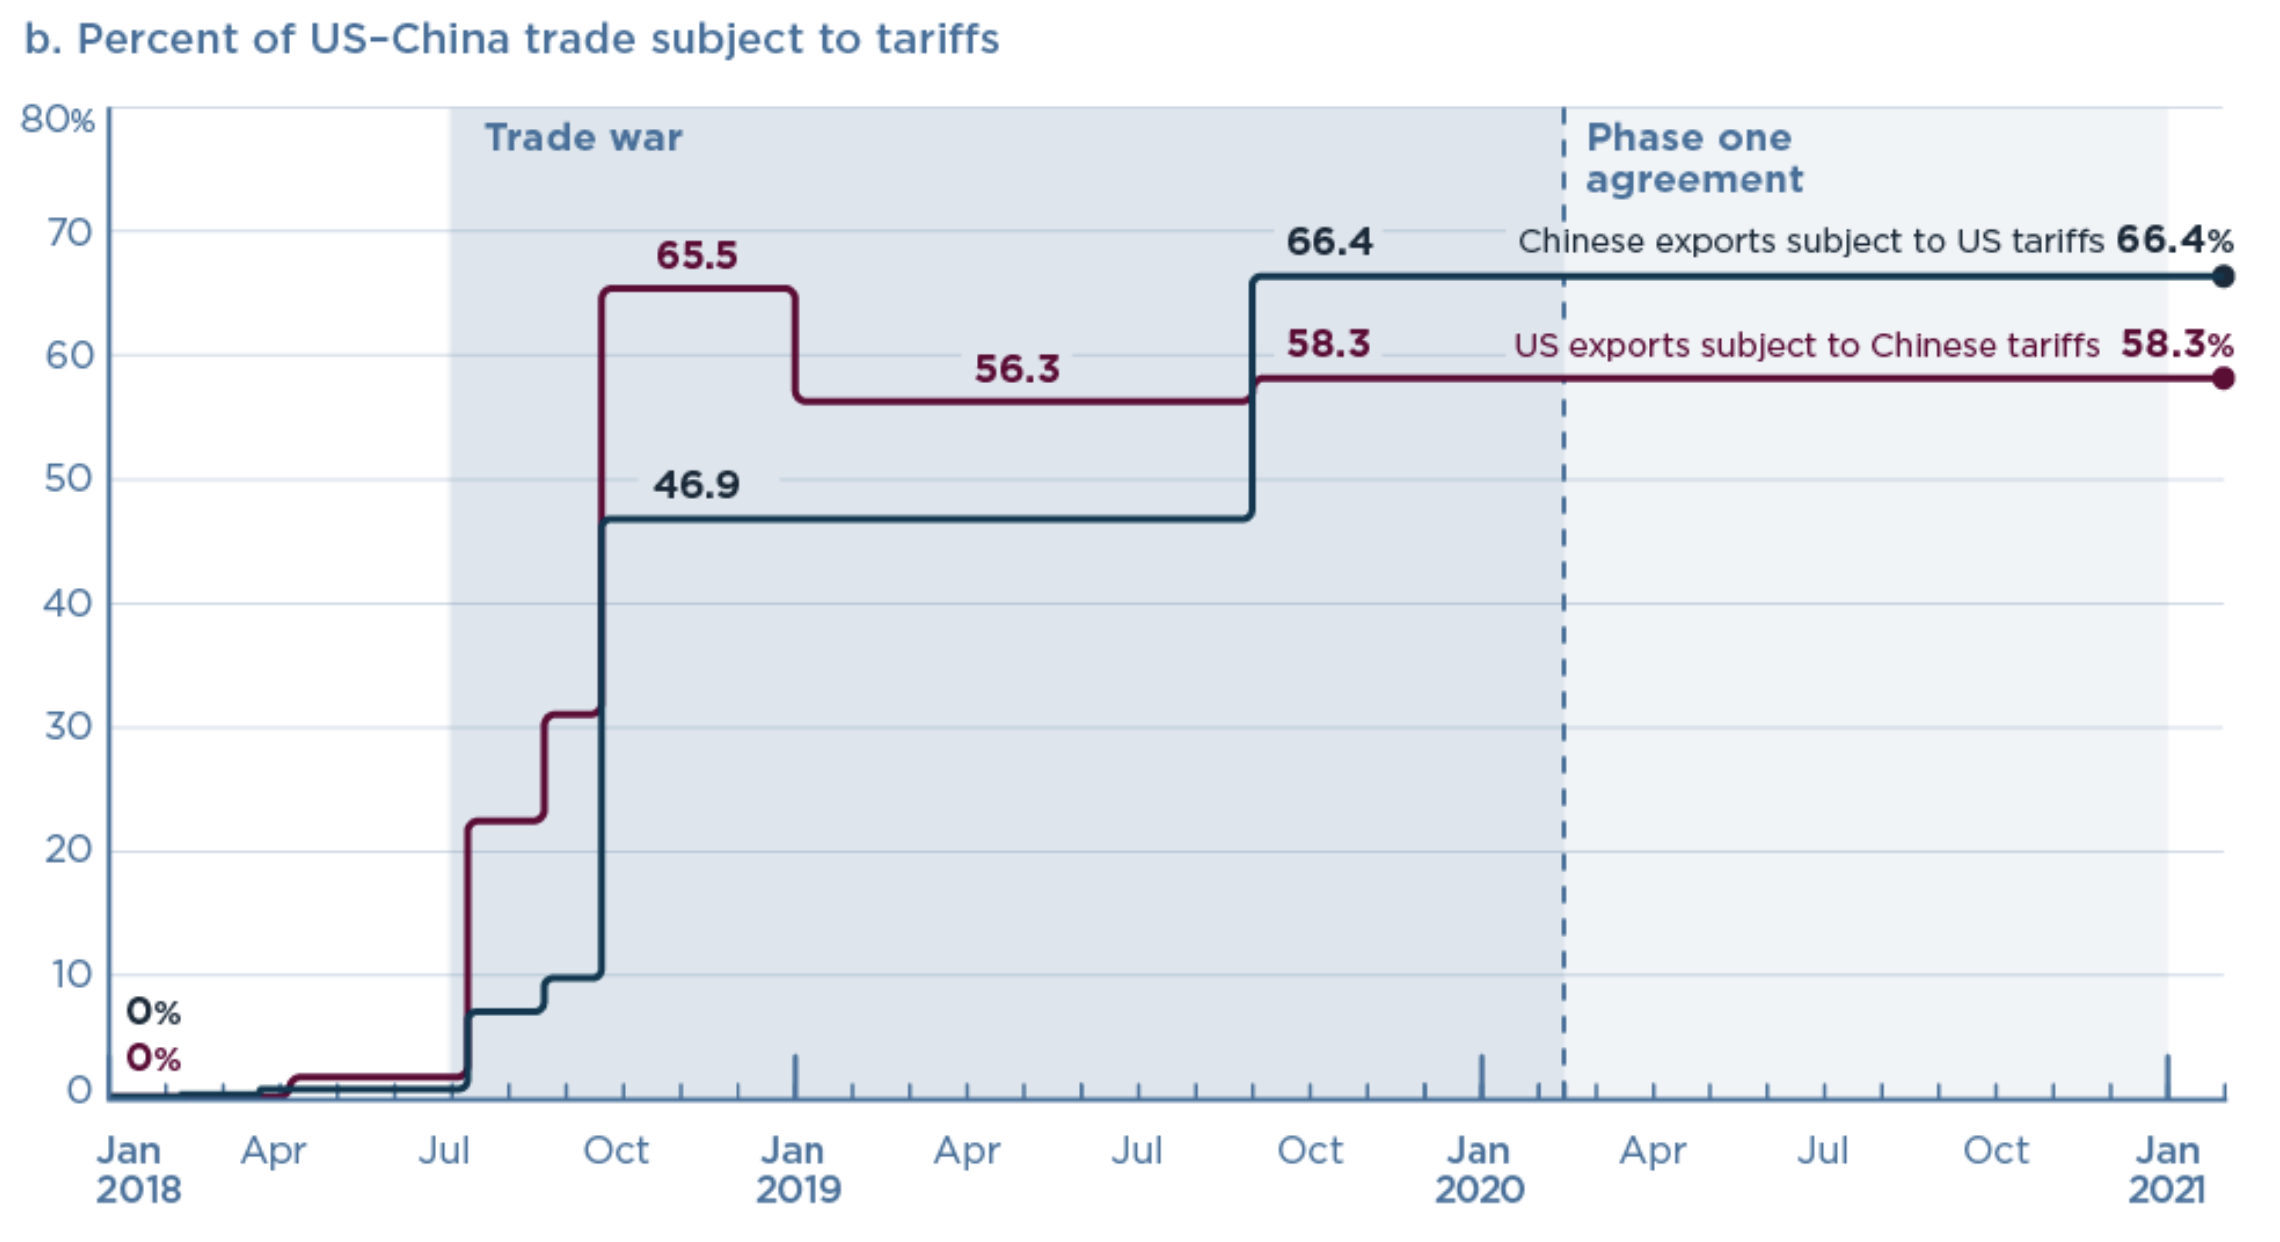
\includegraphics[width=\linewidth]{Scope of Tariffs Trade War.png}
        \caption{Source: \textcite{piie_us_china_trade_war_2023}}
        \label{fig:enter-label}
    \end{figure}
\end{frame}

\begin{frame}{Tariff Levels over Time}
    \begin{figure}
        \centering
        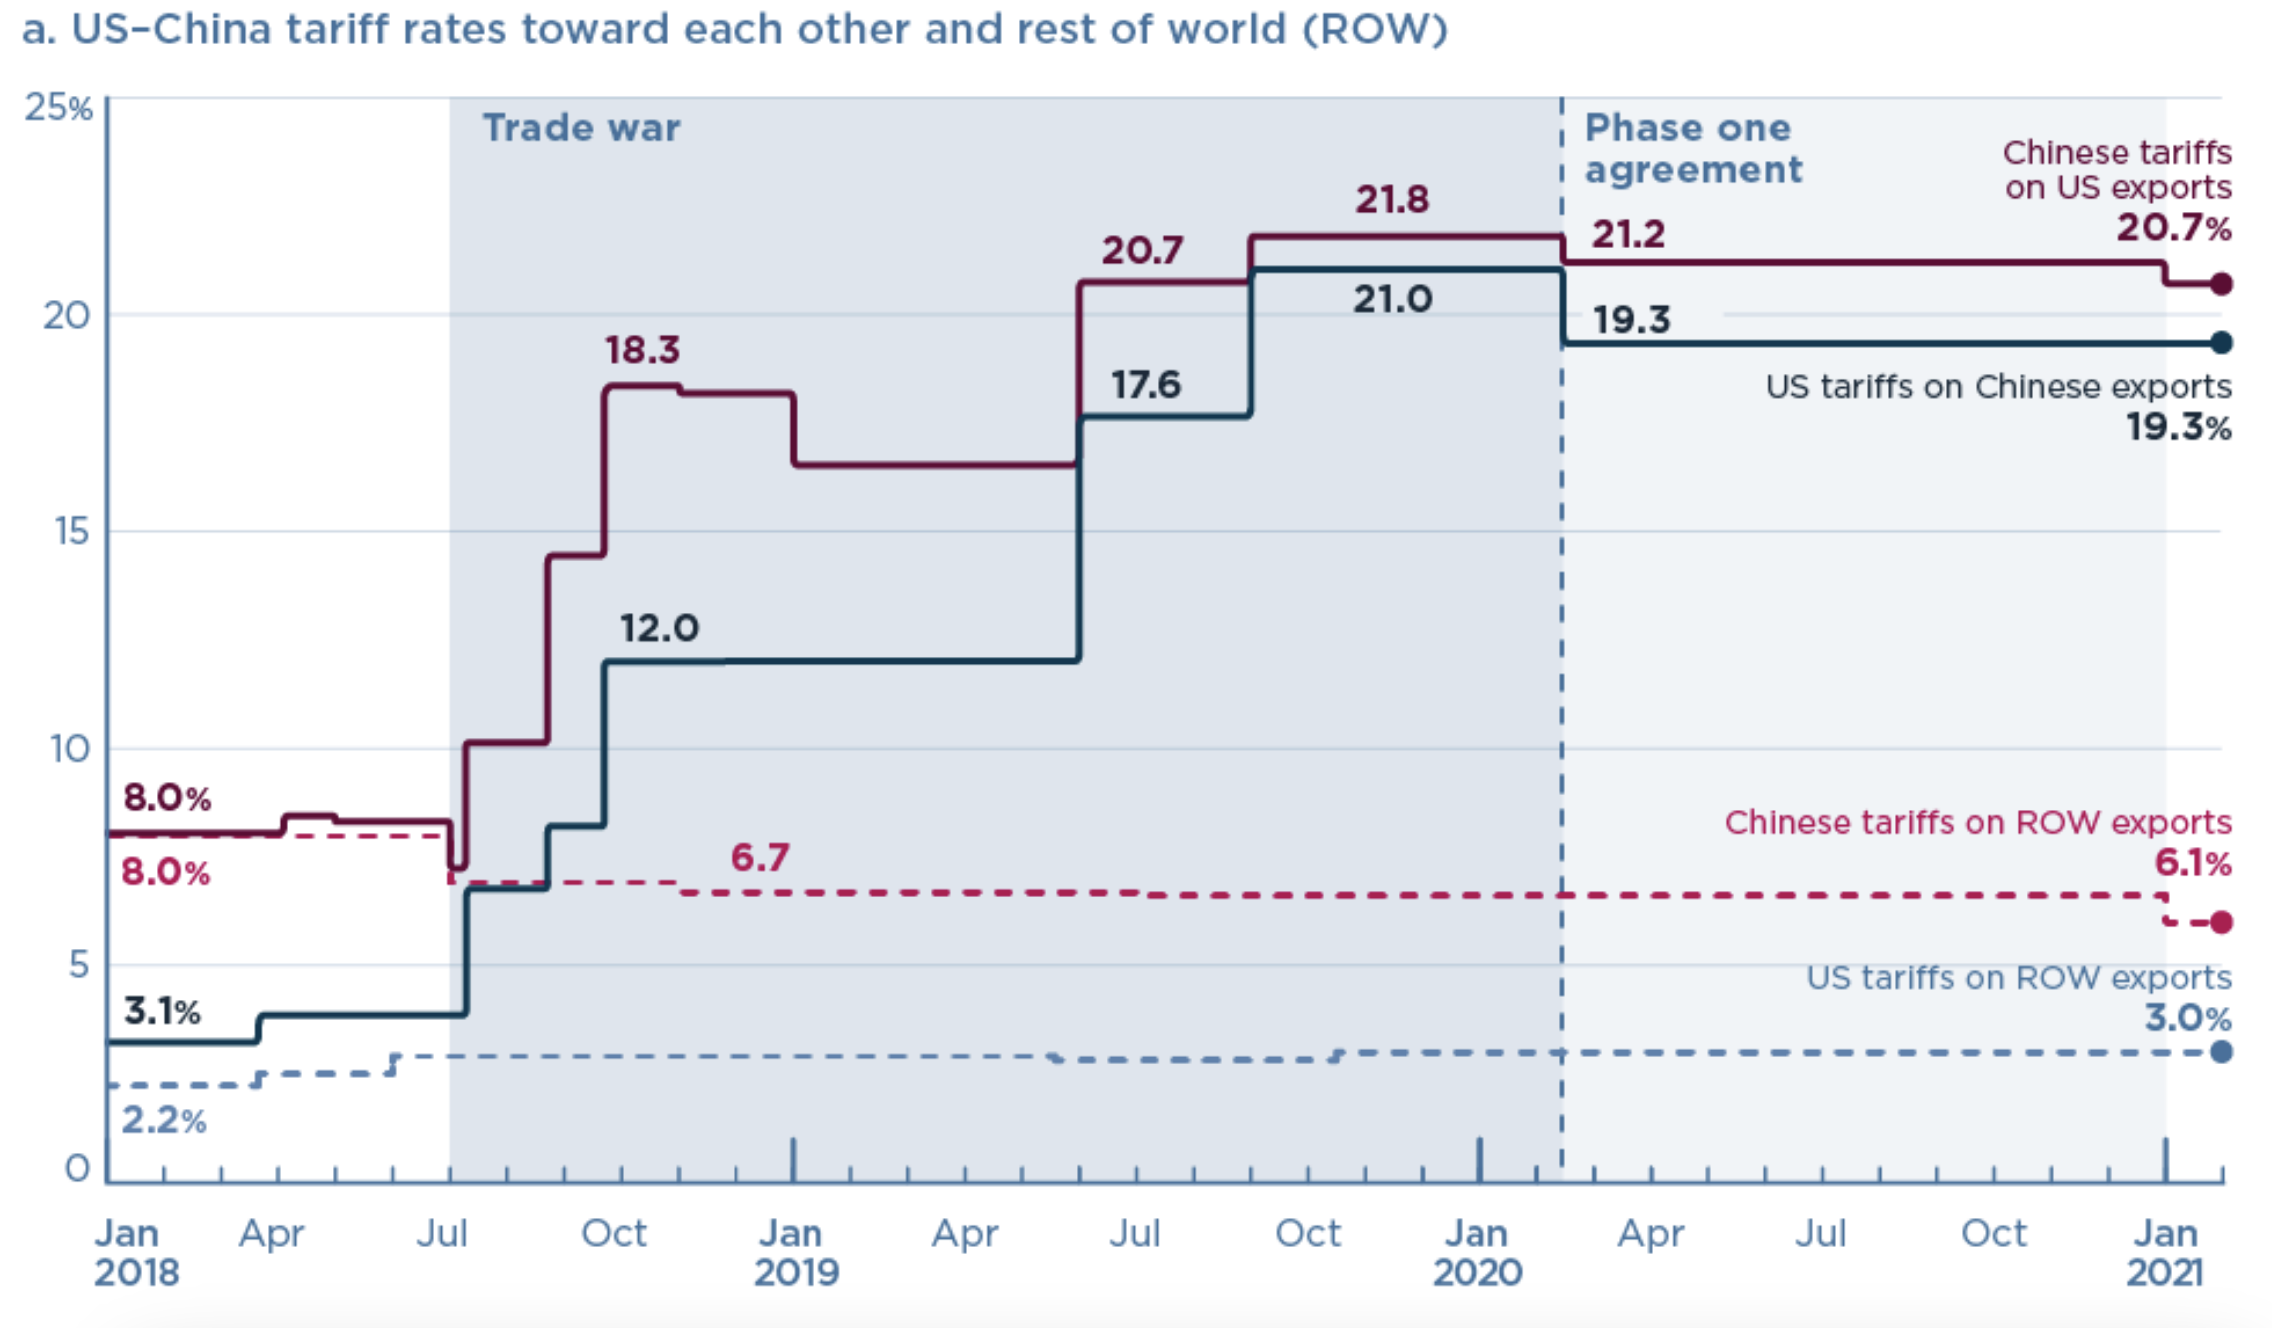
\includegraphics[width=\linewidth]{Tariffs during Trade War.png}
        \caption{Source: \textcite{piie_us_china_trade_war_2023}}
        \label{fig:enter-label}
    \end{figure}
\end{frame}

\begin{frame}{Example: US-China Trade War Impacts}
\textbf{Impact:}
\begin{itemize} \small
    \item \textbf{Economic:}
    \begin{itemize}  \footnotesize
        \item Increased costs for U.S. businesses.
        \item U.S. farmers largely lost access to Chinese markets; China diversified suppliers (e.g., Brazil for soybeans).
        \item Higher prices for U.S. consumers on imported goods.
    \end{itemize}
    \item \textbf{Political:}
    \begin{itemize} \footnotesize
        \item Tensions between the U.S. and China intensified, extending to tech and geopolitics.
        \item Phase One Trade Agreement (2020): China agreed to purchase \$200 billion in U.S. goods over two years.
    \end{itemize} 
    \item \textbf{Global:}
    \begin{itemize} \footnotesize
        \item Other economies (e.g., EU, Japan) caught in crossfire due to supply chain disruptions. % global supply chains are dependent on intermediate goods that are either produced or traded my China and the U.S. - tariffs increase the costs along the way. Trade diversion leads to increased competition in other markets, potentially harming the domestic industry in Latin America. Undermines the authority of the WTO. It is supposed to act as an institution that prevents trade wars from happening. Reeduced demand in both China and the US due to lower disposable income
        \item Some countries benefited (e.g., Vietnam and Brazil). % multinational companies that used to produce in China relocated their manufacturing facilities to Vietnam to not be affected by US tariffs, that lead to an increase in Vietnams income and exports. Brazil was in a good position since agricultural goods that China formerly imported from the US were now imported from Brazil
    \end{itemize}
\end{itemize}
\end{frame}

\begin{frame}{Trade Wars of the Future?}
   \begin{minipage}{0.3\textwidth}
        \centering
        \textcolor{red}{\textbf{Slide from 21.11.2024}} \vspace{0.2cm}\\
        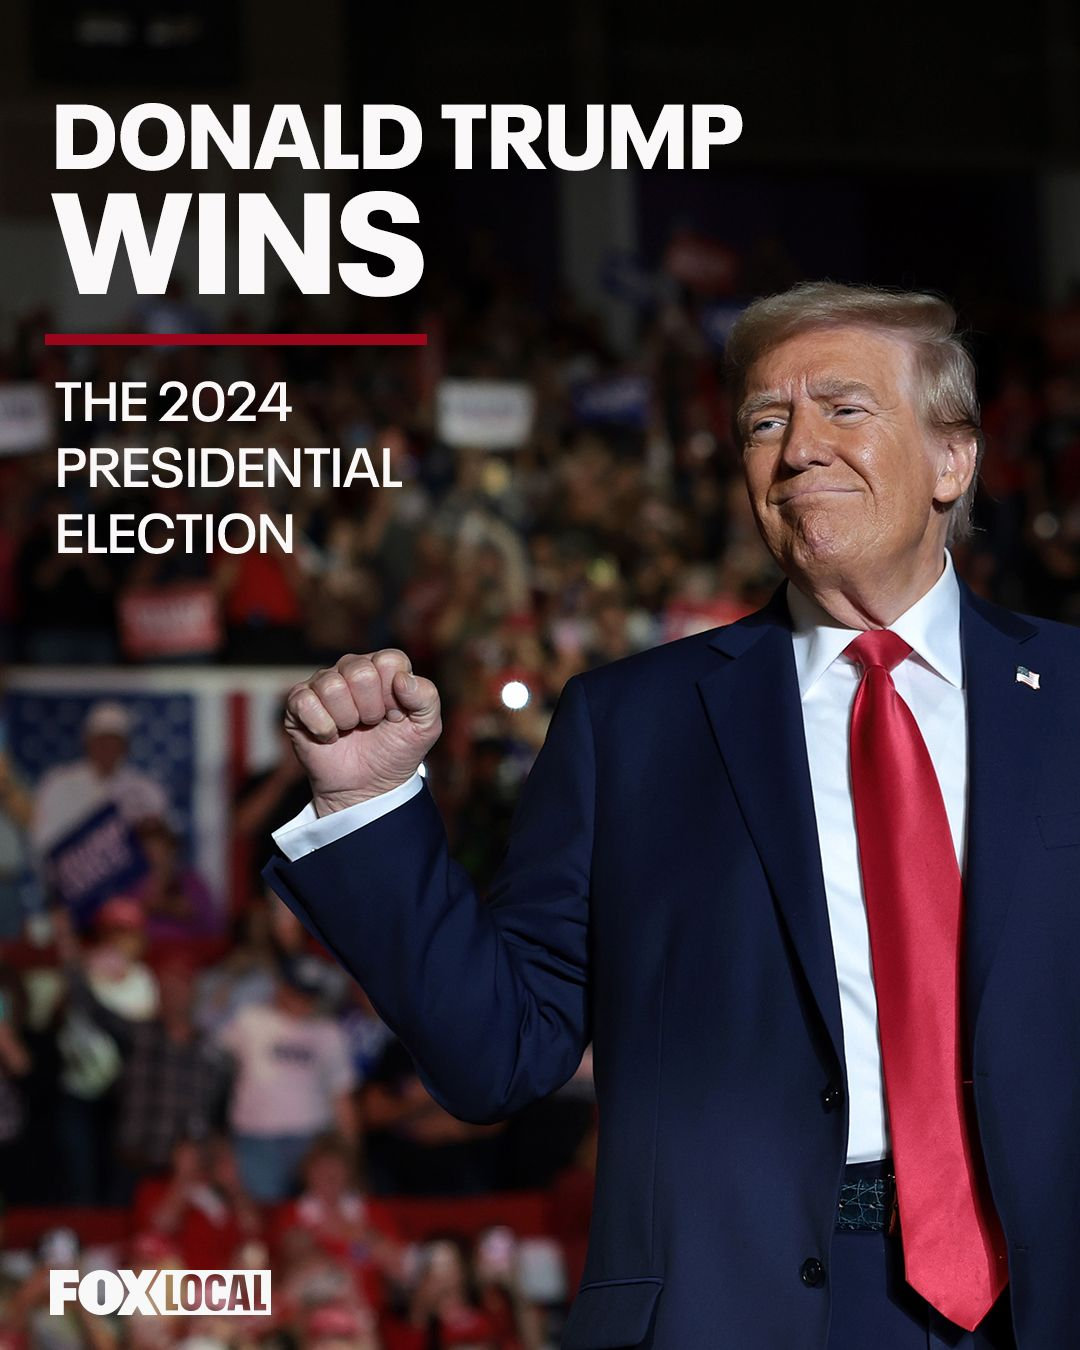
\includegraphics[width=\textwidth]{trump} 
    \end{minipage}%
    \hfill
    \begin{minipage}{0.65\textwidth}
    \textbf{Speculations from polled economists:}
        \begin{itemize}
  \item The average tariff on Chinese goods could be raised by 32–37\%.
  \item Such new U.S. tariffs would reduce China's 2025 economic growth by around 0.5-1.0 percentage point.
  \item Most economists do not expect up to 60\% U.S. tariffs on Chinese goods in early 2025 as this could accelerate inflation in the U.S.
        \end{itemize}
    \end{minipage}
\end{frame}

\begin{frame}{US-China Trade War 2.0}
    \begin{figure}
        \centering
        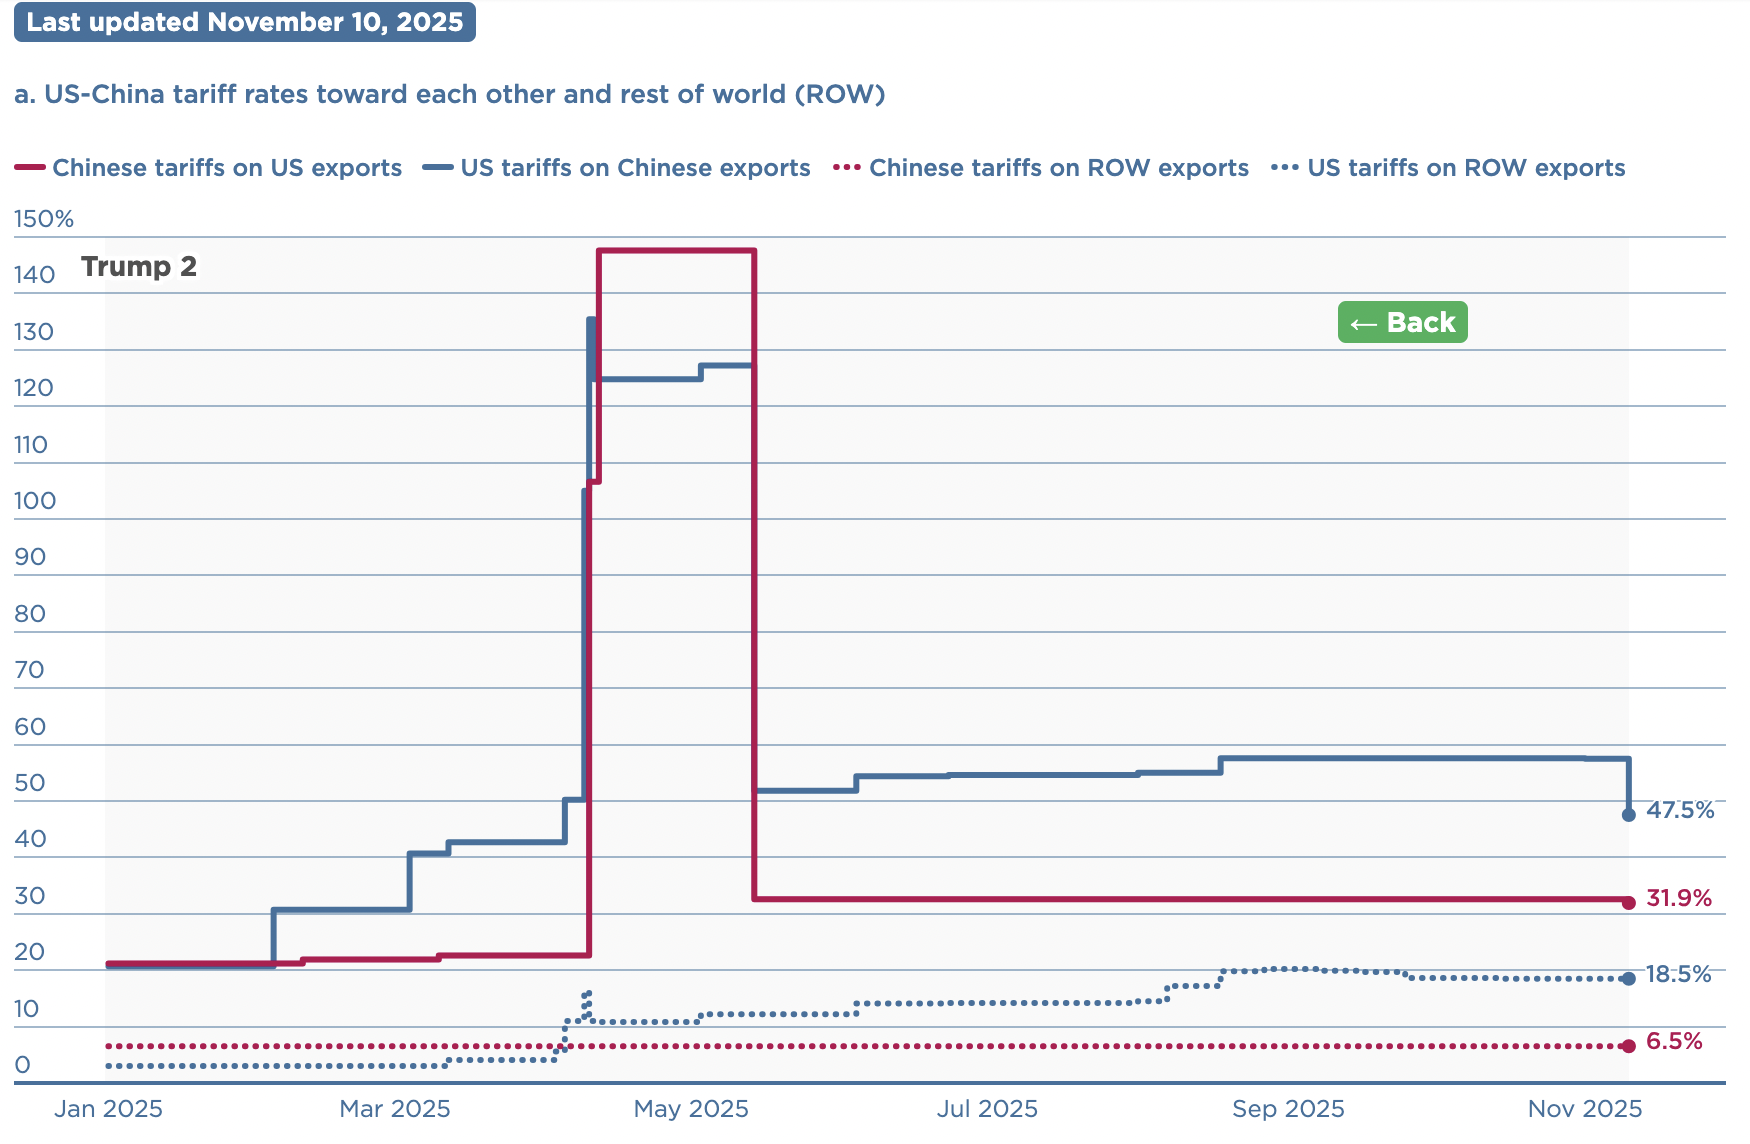
\includegraphics[width=0.9\linewidth]{trade war 2.0.png}
        \caption{Source: \textcite{piie_us_china_trade_war_2025}}
        \label{fig:placeholder}
    \end{figure}
\end{frame}



\begin{frame}[allowframebreaks]{References}
    \printbibliography
\end{frame}


\end{document}

